\documentclass[\report.tex]{subfiles}
\begin{document}

\section{Appendices}

\subsection{Appendix 1.0 - SfePy}
Simple finite elements in Python (SfePy) uses finite element methods to solve coupled partial differential equation (PDE) in systems up to three dimensions. SfePy is a powerful software that allows complex physical problems to be coded quickly and easily. It has been used successfully in a variety of disciplines, ranging from biomechanical modelling \cite{biomedapplication} to the computational analysis of acoustic transmission coefficients \cite{AcousticTransmission}.\\ \\In this report, the input file to the SfePy software is a microstructural image which must first be 'cleaned' through segmentation, mesh generation and noise reduction. It can then be imported into the software as a mesh file, where boundary and initial conditions are applied. Fields are then created which can be used to define variables which may be 'unknown field', 'test field' or 'parameter field' \cite{FEMinSfePy} and the material properties are defined. Complications arose in attempting to use SfePy for the processed images, therefore the group opted to use the OOF2 FEM software instead.

\begin{figure}[h!]
    \centering
    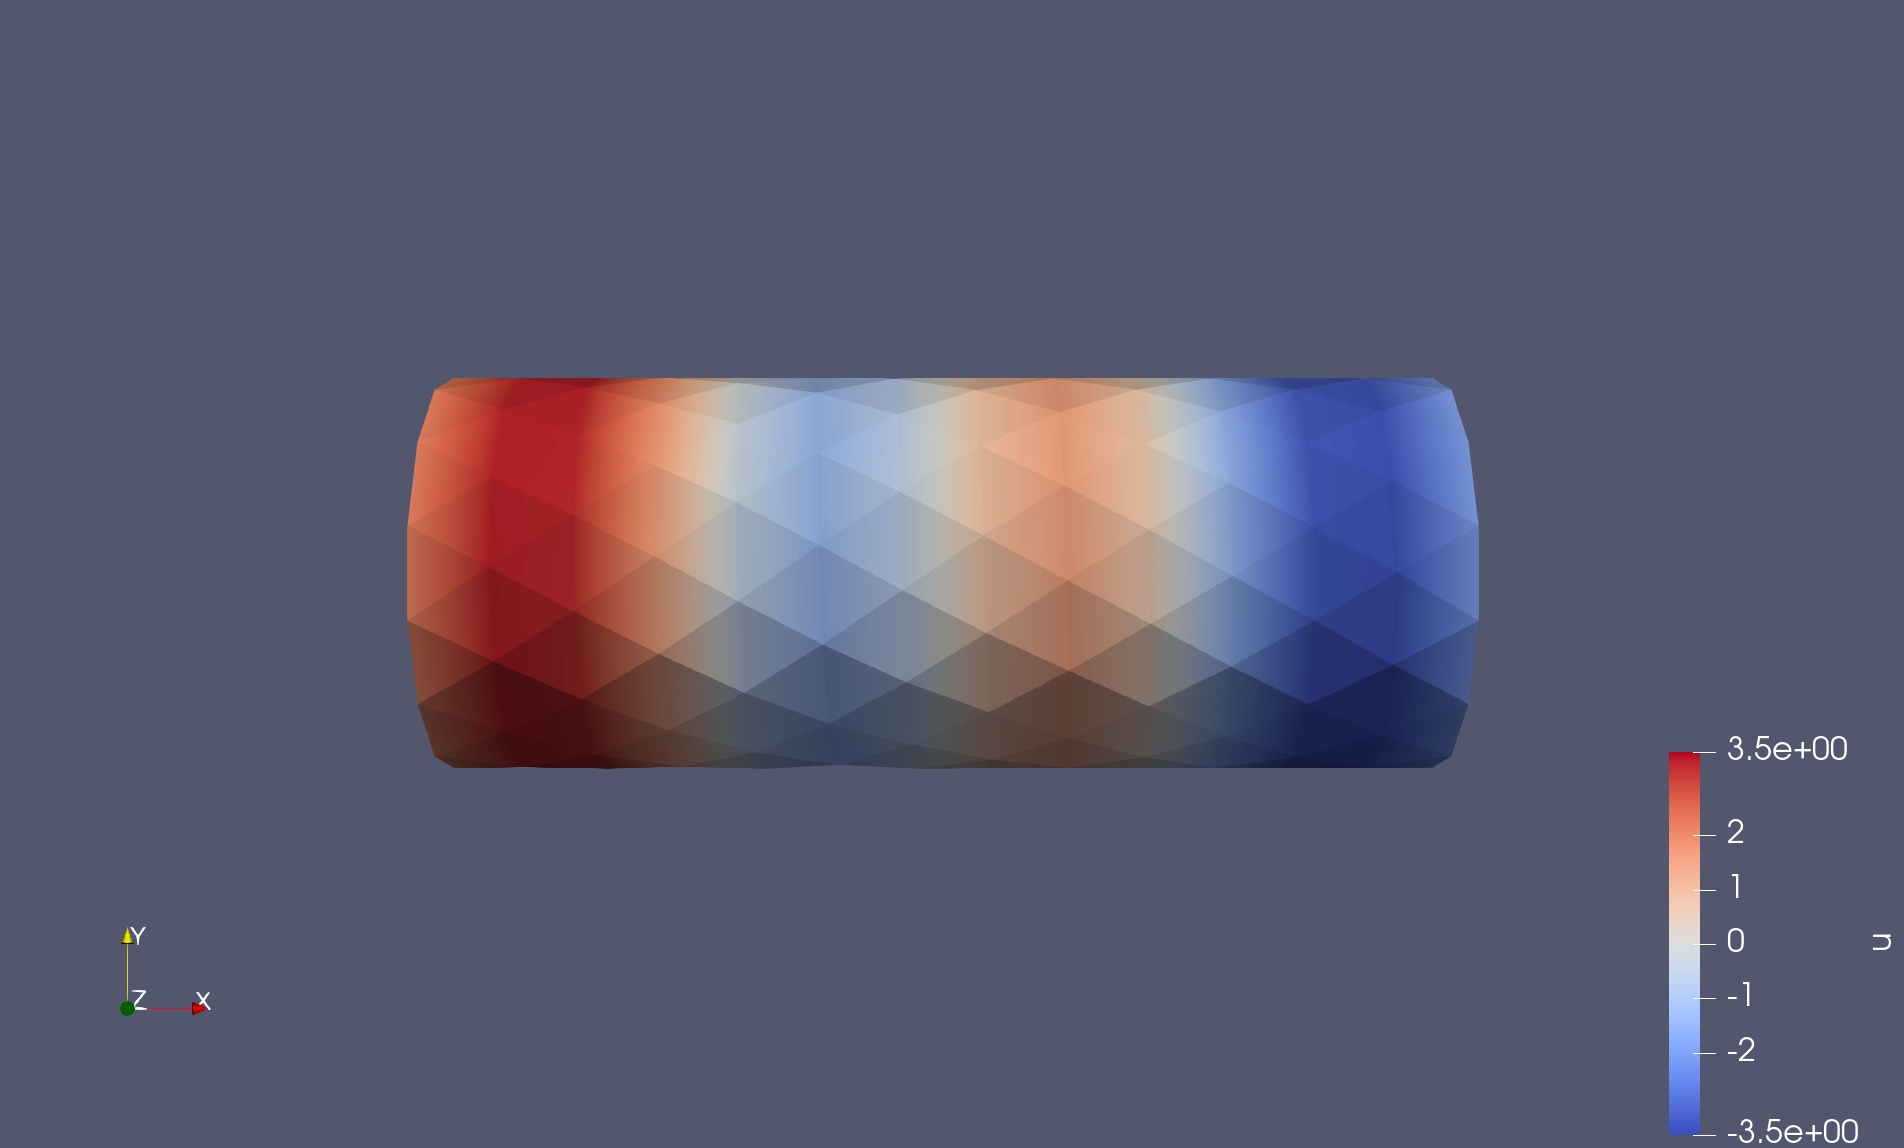
\includegraphics[width=14cm]{Images/cylinder_diffusion.png}
    \caption{Gmsh adaptive mesh generated for image: cylinder\_diffusion.png}
    \label{fig:sfepy_example}
\end{figure}


\subsection{Appendix 2.0 - Gmsh}
Gmsh is a tool for creating a finite element mesh from an image or a geometry built from scratch. The software allows for editing of algorithm scripts based in ASCII to finely tune node and element positions or even adaptively mesh. This was originally used to create input files for SfePy, however OOF2 was chosen instead. Figure~\ref{fig:gmsh} shows an example of a adaptive generated mesh for one of the images.

\begin{figure}[h!]
    \centering
    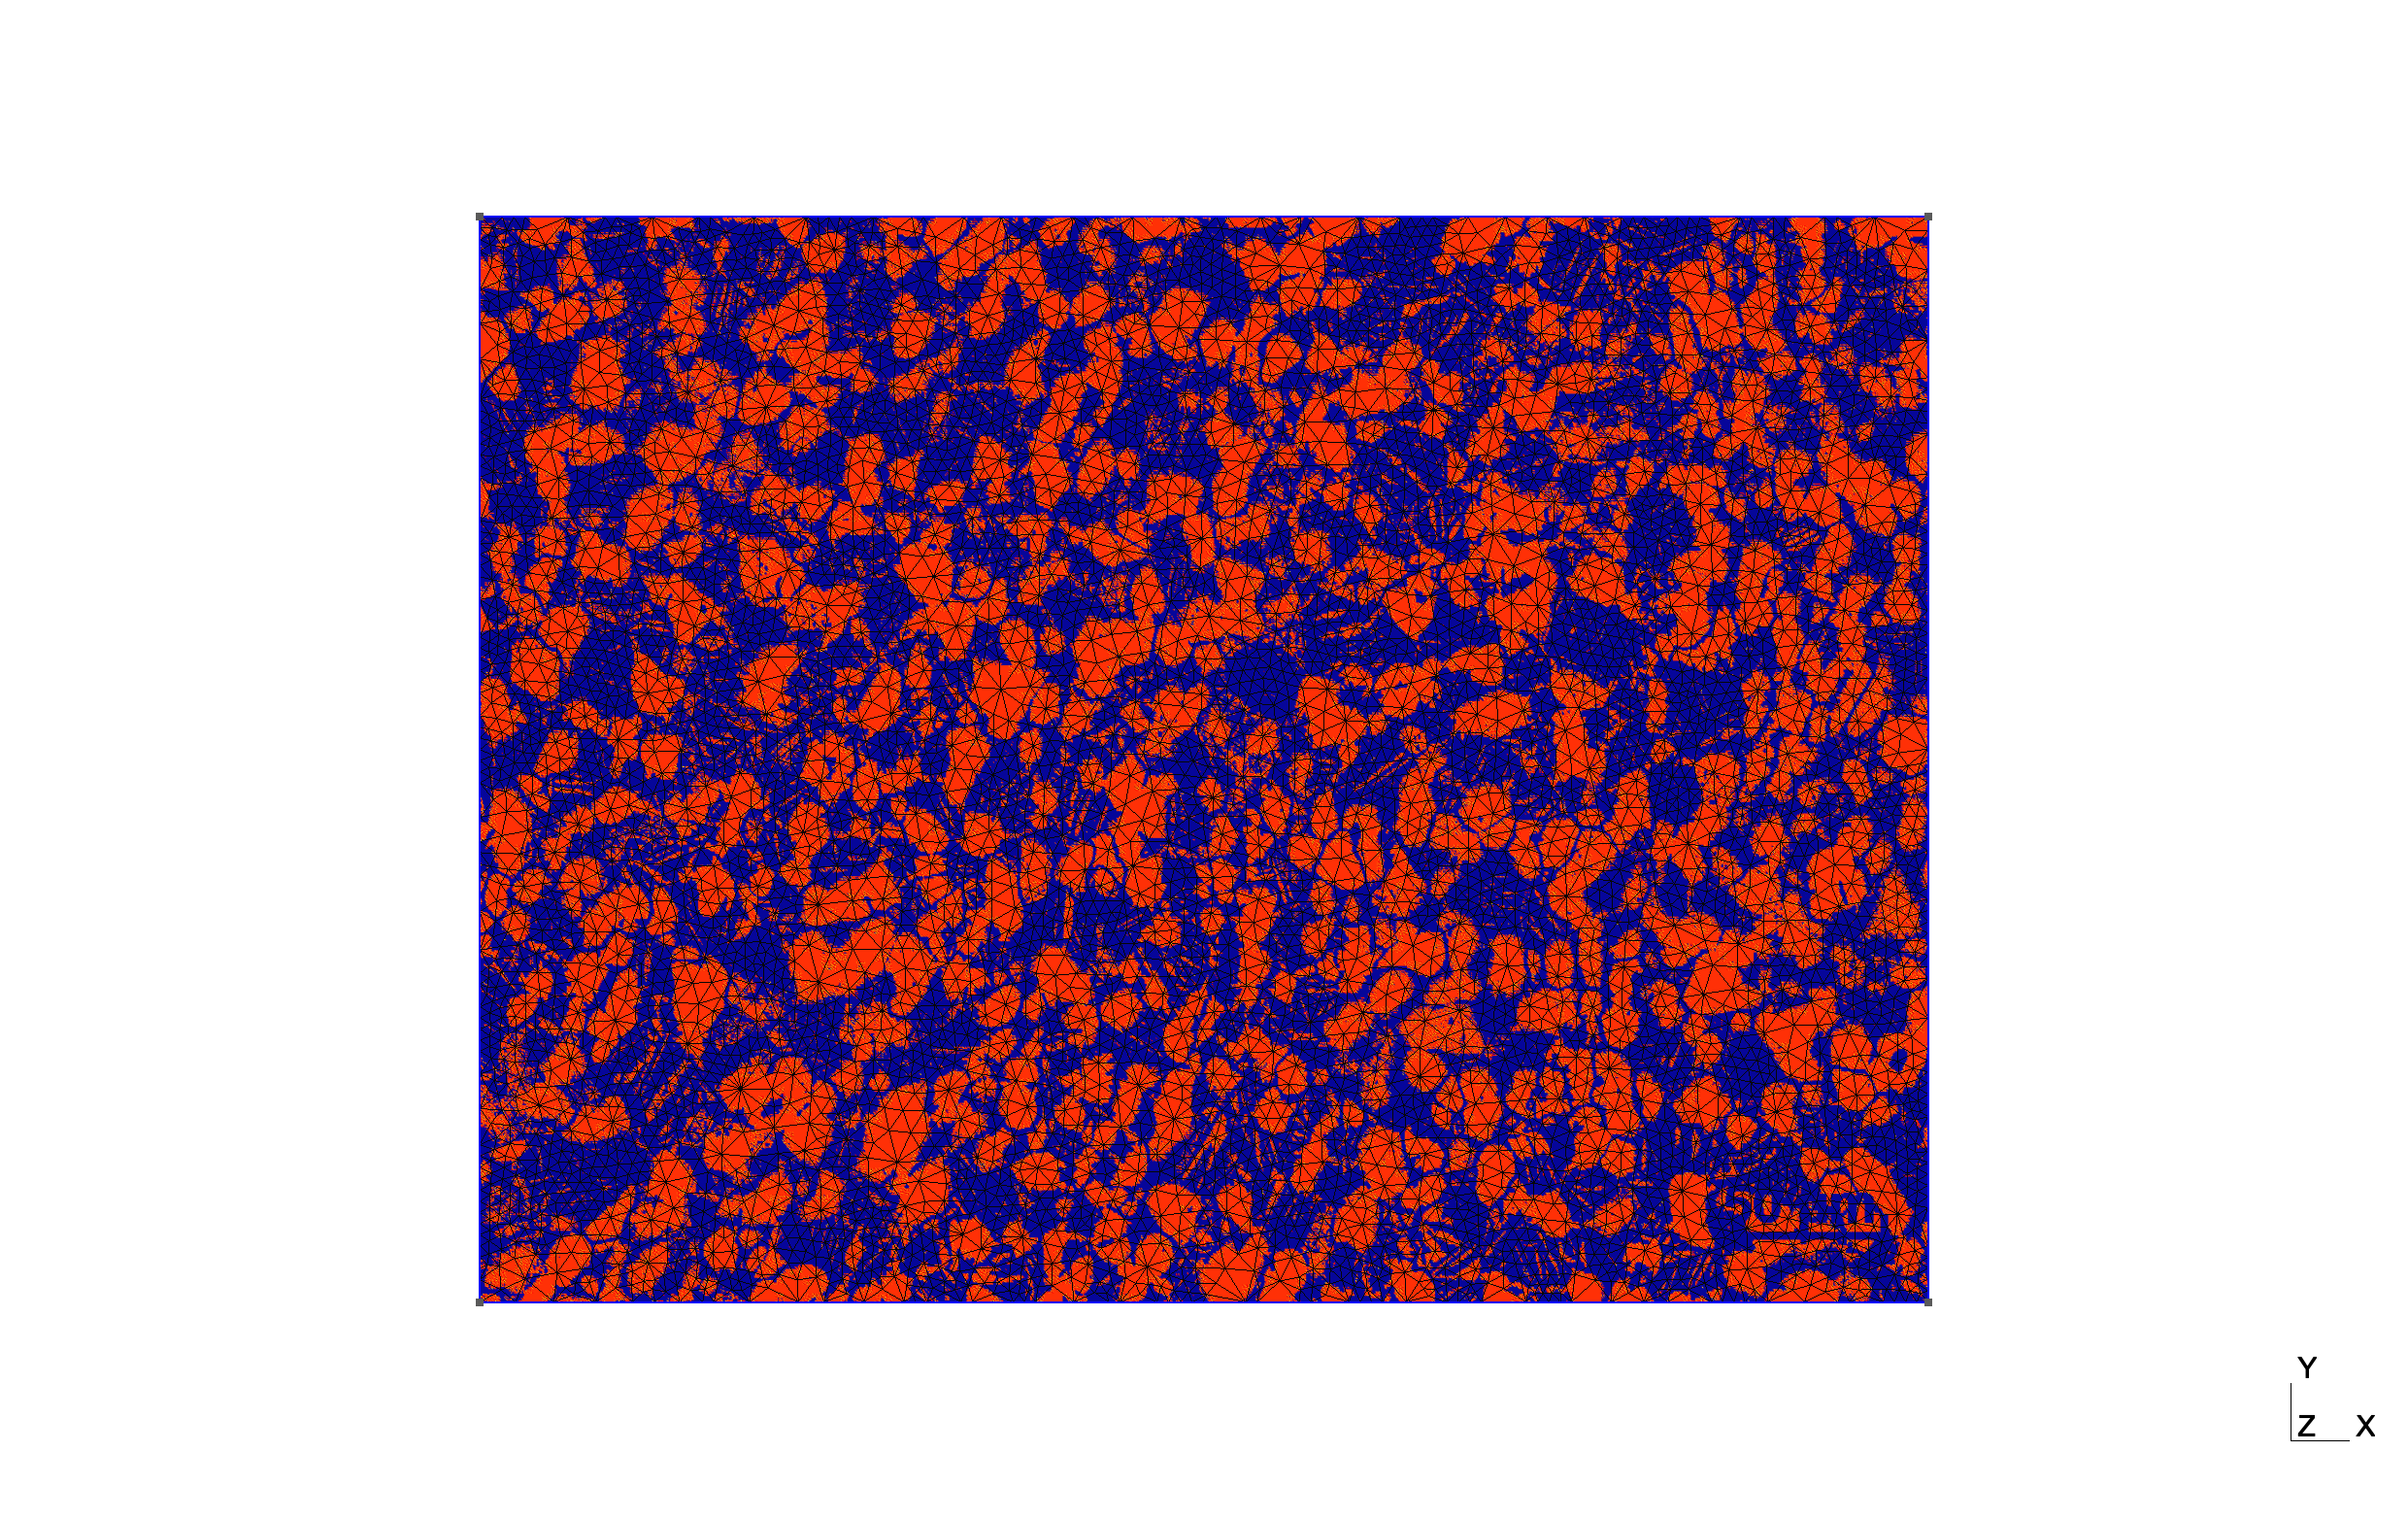
\includegraphics[width=14cm]{Images/out.png}
    \caption{Gmsh adaptive mesh generated for image: Ti64BFi20xbinary.png}
    \label{fig:gmsh}
\end{figure}

\end{document}
